%\documentclass[italian]{scrreprt}
\documentclass[italian,a4paper,12pt,oneside]{book}
\usepackage[T1]{fontenc}
\usepackage[utf8]{inputenc}
\usepackage{geometry}
\usepackage{graphicx}
\usepackage{forest}
\setcounter{secnumdepth}{3}
\setcounter{tocdepth}{1}
\usepackage{float}
\usepackage{babel}
\usepackage{microtype} % migliora espansione dei font. Suggerito su ``L'arte di scrivere in LaTeX, pag. 45''
\usepackage{indentfirst} % indentazione anche su primo paragrafo.  Suggerito su ``L'arte di scrivere in LaTeX, pag. 45''
\usepackage{booktabs} % serve per le tabelle.   Suggerito su ``L'arte di scrivere in LaTeX, pag. 85''
\usepackage{caption} % serve per le tabelle.   Suggerito su ``L'arte di scrivere in LaTeX, pag. 85''



\geometry{textheight=24.2cm,textwidth=16cm}
\pagestyle{headings}
\frenchspacing

\date{}

\title{
\huge Guida all'uso della piattaforma di prenotazione sale
\\ Booked
} 
\author{Revisione 0.08 \\
Germano Massullo}

\makeindex

\begin{document}
\frontmatter		% inizia la numerazione con numeri romani

\maketitle
\tableofcontents
\mainmatter		% inizia la numerazione con numeri cardinali
\chapter{Introduzione}
La presente guida ha come oggetto l'utilizzo della piattaforma Booked scheduler
per gestione elettronica delle prenotazioni di aule dell'ateneo.
Per un'agevole comprensione del testo, vengono introdotti di seguito alcuni concetti preliminari.
Booked gestisce tre tipi fondamentali di oggetti:
\begin{itemize}
 \item calendari;
 \item risorse;
 \item prenotazioni.
\end{itemize}
\paragraph*{Calendari}\mbox{}\\ %per andare a capo dopo nome paragrafo.
I calendari presenti sono:
\begin{itemize}
 \item Default;
 \item Economia;
 \item Ingegneria;
 \item Lettere;
 \item Medicina;
 \item Scienze.
\end{itemize}

in maniera tale da separare le esigenze di prenotazione delle varie macro aree d'ateneo.
Il calendario ``Default'' è un calendario predefinito e vuoto, che appare quando si accede
alla pagina web dei calendari, pertanto occorre scegliere quello di propria competenza.

\paragraph*{Risorse}\mbox{}\\ %per andare a capo dopo nome paragrafo.
Booked gestisce prenotazioni di risorse: esse possono essere laboratori, laboratori,
mezzi di trasporto, aule didattiche, ecc. Queste ultime pertanto, verranno viste dal
programma come delle risorse.


\paragraph*{Prenotazioni}\mbox{}\\ %per andare a capo dopo nome paragrafo.
Le prenotazioni vengono effettuate operando sulla pagina che mostra il calendario: si sceglie
la risorsa da prenotare e si impostano le proprie preferenze.
\chapter{Prenotazioni}
Per effettuare una prenotazione, cliccare la voce ``Calendario'' nel menù in alto alla pagina web.
Selezionare il calendario di propria competenza
\begin{figure}[H]
\centering{}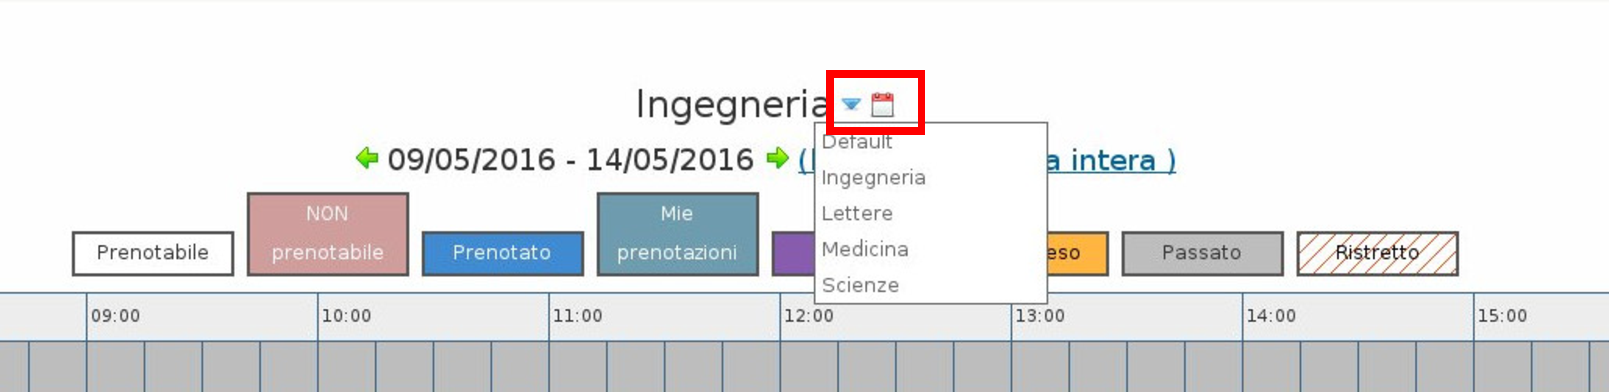
\includegraphics[scale=0.5]{Immagini/calendari_selezione.pdf}
\normalsize
\caption{}
\label{fig:calendari_selezione.pdf}
\end{figure}

e scorrere la pagina fino a trovare la data adatta alla prenotazione. Sulle righe
sono presenti tutte le risorse (aule) disponibili.
Per iniziare a creare una prenotazione cliccare su un quadratino qualsiasi nella fascia oraria
dell'aula desiderata. È possibile modificare i dettagli orari nella schermata
successiva.

Per fissare una prenotazione su più giorni della settimana, andare nella zona ``Ripeti'' come in Figura
\ref{fig:prenotazione_ripetizione_1.pdf}

\begin{figure}[H]
\centering{}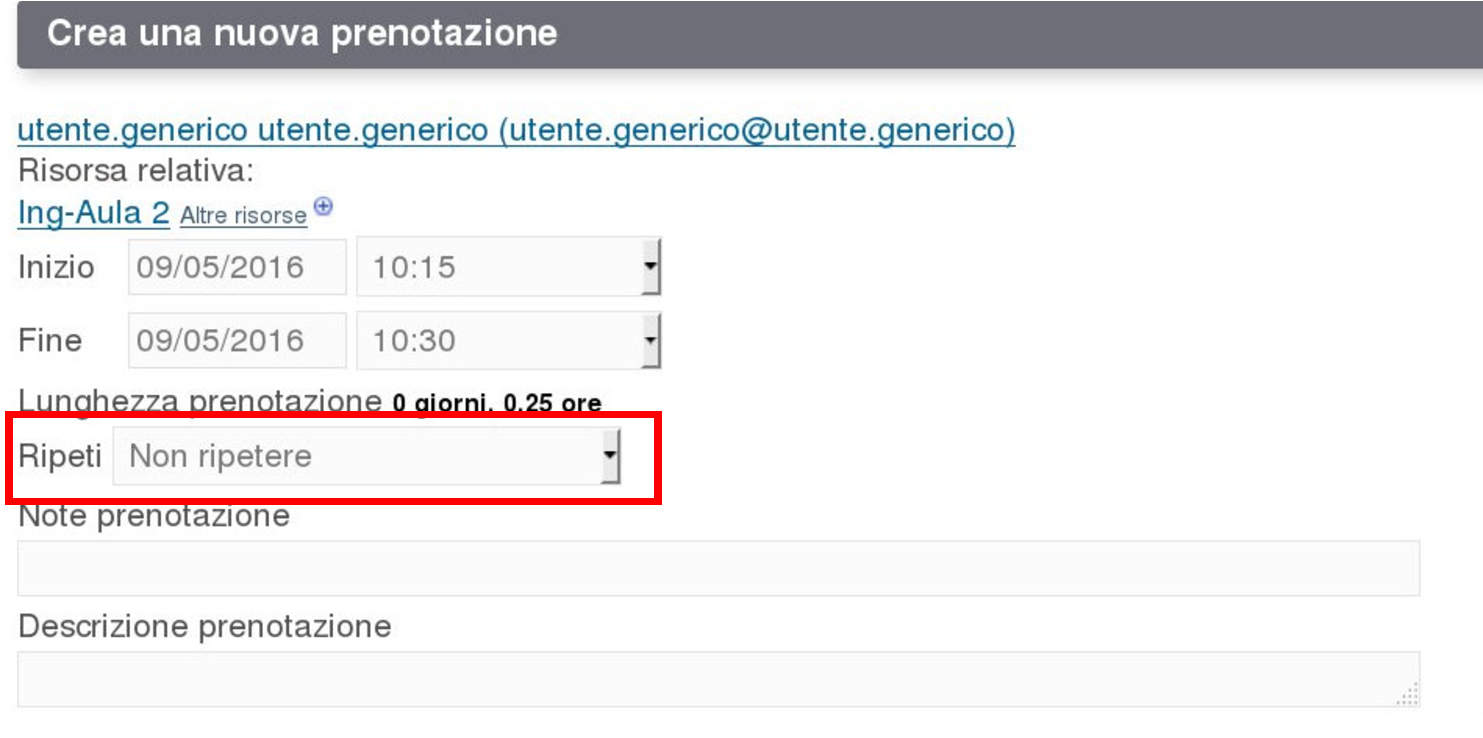
\includegraphics[scale=0.5]{Immagini/prenotazione_ripetizione_1.pdf}
\normalsize
\caption{}
\label{fig:prenotazione_ripetizione_1.pdf}
\end{figure}

e cliccare su ``Settimanale''

\begin{figure}[H]
\centering{}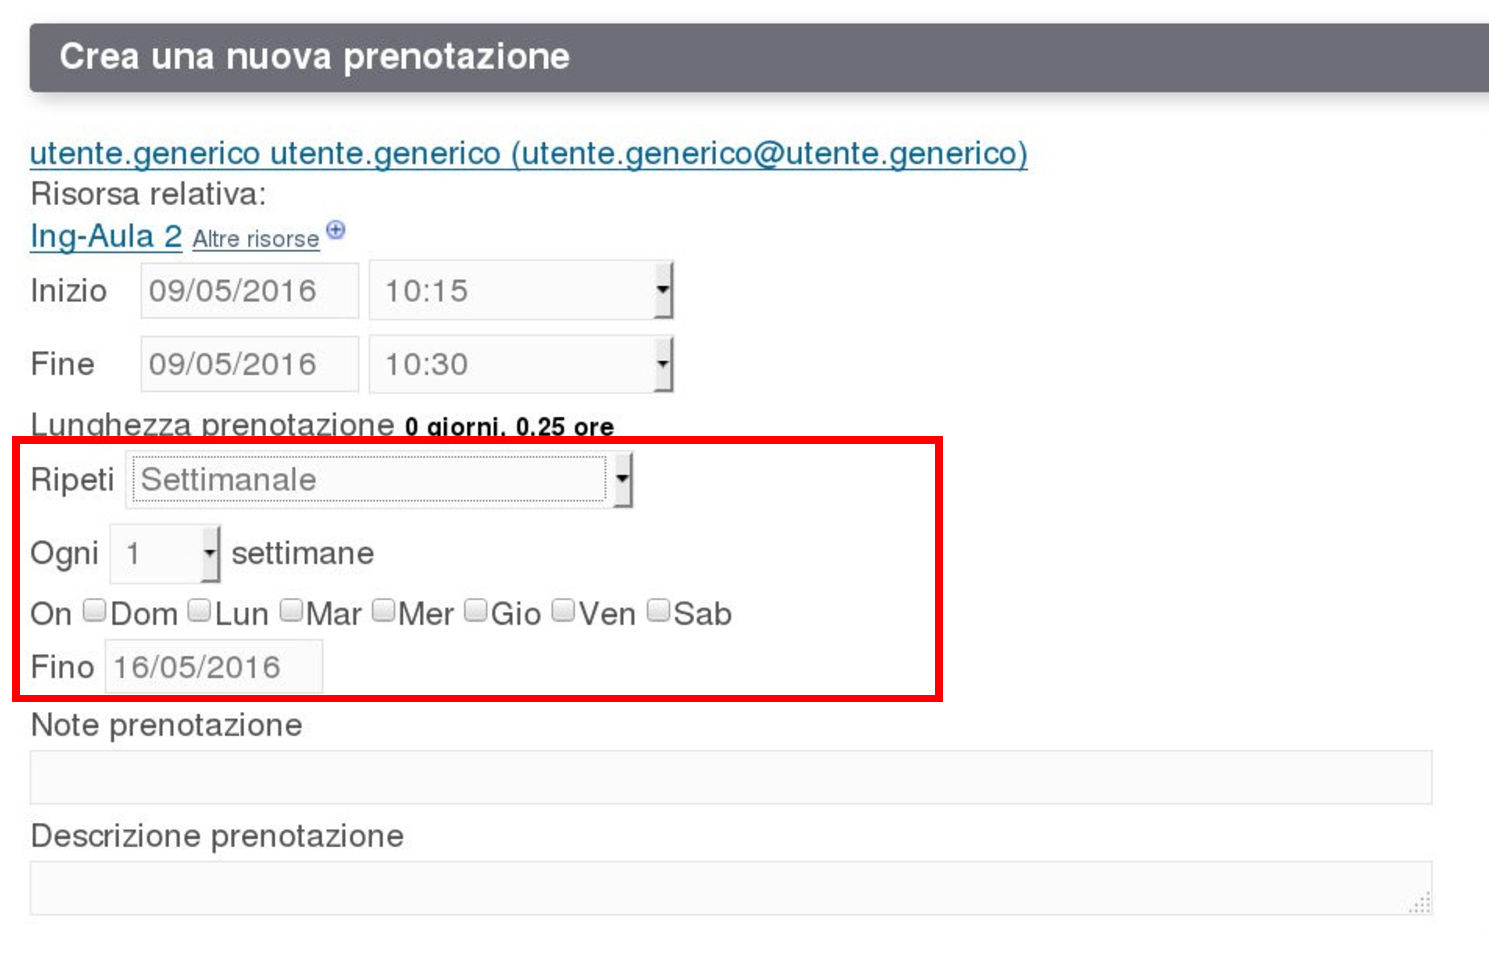
\includegraphics[scale=0.5]{Immagini/prenotazione_ripetizione_2.pdf}
\normalsize
\caption{}
\label{fig:prenotazione_ripetizione_2.pdf}
\end{figure}


La scritta ``Note prenotazione'' significa ``Nome prenotazione''. Vi è un errore di traduzione
del software, che verrà corretto a breve.
Non dimenticare di aggiungere il corso di studi della materia e l'anno corrispondente.


\begin{figure}[H]
\centering{}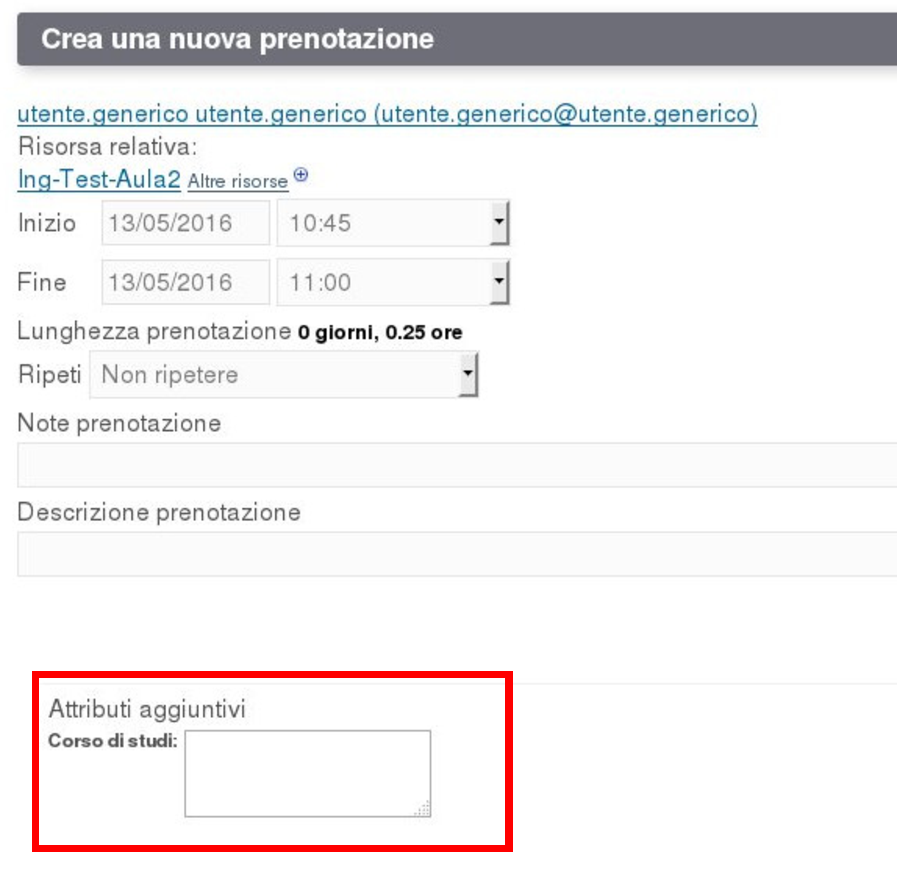
\includegraphics[scale=0.5]{Immagini/prenotazione_attributi.pdf}
\normalsize
\caption{}
\label{fig:prenotazione_attributi.pdf}
\end{figure}

Un esempio può essere

\begin{figure}[H]
 \centering{} Ingegneria informatica II anno
\normalsize
\end{figure}

Nel caso la prenotazione riguardi più corsi di studi, metterne uno per riga
\chapter{Note di revisione}
Di seguito sono specificati i cambiamenti per ogni numero di revisione
della guida
\begin{itemize}
 \item 0.06 aggiunta nomenclatura aule per edificio
 \item 0.07 aggiunto corretto utilizzo campo ``Nome prenotazione''
 \item 0.08 aggiunta spiegazione su come impostare capacità aula/risorsa. Aggiunte note di revisione
\end{itemize}

\end{document}
